\documentclass[letterpaper, 12pt]{article}

\usepackage[utf8]{inputenc}
\usepackage[english, spanish]{babel}
\usepackage{fullpage}
\usepackage{graphicx}
\usepackage{amsmath}
\usepackage{enumitem}
\usepackage{chngcntr}
\usepackage{setspace}
\usepackage{url}
\usepackage{csquotes}
\usepackage{float}
\usepackage{verbatim}
\usepackage{tabularx}
\usepackage{amsmath}
\usepackage{caption}
\usepackage{bm}
\usepackage{colortbl}
\usepackage{xcolor}
\usepackage{multicol}

\usepackage{multirow}

% \usepackage{hyperref}

\counterwithin{figure}{section}
\renewcommand{\thesection}{\arabic{section}}
\renewcommand{\thesubsection}{\thesection.\arabic{subsection}}
\renewcommand{\baselinestretch}{1.5}

\usepackage[style=numeric, maxnames=6, minnames=3, backend=biber, parentracker=true, sorting=none]{biblatex}
\DefineBibliographyStrings{english}{%chktex-file 1 chktex-file 6
      andothers = {\em et\addabbrvspace al\adddot}
}
\addbibresource{./Bibliography/bibliography.bib}

\usepackage{array}

\setlength{\parskip}{0pt}

\raggedbottom{}

\newcommand{\bolditalic}[1]{\textbf{\textit{#1}}}

\begin{document}

\begin{titlepage}
      \centering
      
\includegraphics[width=0.3\textwidth]{Images/logo_utb.png}\par\vspace{1cm}
      {\scshape\LARGE Universidad Tecnológica de Bolívar \par}
      \vspace{1cm}

      {\scshape\Large FÍSICA CALOR Y ONDAS \par}
      \vspace{.2cm}

      % chktex-file 8
      {\scshape\Large Grupo 1 \par}
      \vspace{1cm}
      % chktex-file 8
      \slshape {\Large \bfseries{}Informe de Laboratorio No. VII\\}
      \slshape {\small \bfseries{}EFECTO FOTOELÉCTRICO}
      \vspace{2cm}

      \slshape {\itshape{} Mauro González, T00067622 \\}
      \slshape {\itshape{} German De Armas Castaño, T00068765 \\}
      \slshape {\itshape{} Angel Vega Rodriguez, T00068186 \\}
      \slshape {\itshape{} Juan Jose Osorio Ariza, T00067316 \\}
      \slshape {\itshape{} Jorge Alberto Rueda Salgado, T00068722 \\}
      \vfill
      Revisado Por \\
      Duban Andres Paternina Verona\\
      {\large \today\par}
\end{titlepage}

% chktex-file 44
% chktex-file 24

% ! ----------------------------------------------------------------------|>
\section{Introducción}

El efecto fotoeléctrico está estrechamente ligado al
fenómeno dual de la materia, que se manifiesta tanto como
onda y partícula. En el marco de la física clásica, esta
dualidad del comportamiento de la materia, especialmente en
relación con la luz, no podía ser plenamente comprendida.
Es esencial tener en cuenta que, gracias a las aplicaciones
del efecto fotoeléctrico, que marcó el inicio de la
mecánica cuántica, hemos podido desarrollar dispositivos e
instrumentos que serían inutilizables o inapreciables sin
este fenómeno.

En esta experiencia de laboratorio, nos centraremos en la
exploración y comprobación de los conceptos relacionados
con los fundamentos del efecto fotoeléctrico la frecuencia
de la luz incidente, el comportamiento de los electrones y
el límite de tensión marcado a la hora de extraer
electrones.

% ! ----------------------------------------------------------------------|>
\section{Objetivos}

% + -------------------------------------------------------------|>
\subsection{Objetivo general}

Comprobar de manera experimental la ecuación de Einstein en
el contexto del efecto foto eléctrico.

% + -------------------------------------------------------------|>
\subsection{Objetivos específicos}

\begin{itemize}
      \item Calcular la constante de Planck ($h$) y la función de
            trabajo ($W_o$) de la celda fotoeléctrica
      \item Evidenciar cómo el efecto fotoeléctrico puede ser utilizado
            para comprender la naturaleza de partículas de la radiación
            electromagnética
\end{itemize}

% ! ----------------------------------------------------------------------|>
\section{Marco Teórico}

% + -------------------------------------------------------------|>
\subsection{Efecto fotoeléctrico~\cite{efecto_fotoelectrico_1}~\cite{efecto_fotoelectrico_2}}

El efecto fotoeléctrico, también denominado fotoemisión, se
refiere al fenómeno en el cual la superficie de un metal es
iluminada por luz, lo que resulta en la expulsión de
electrones. Es importante destacar que, en términos de
propiedades y comportamiento, los fotoelectrones no
presentan distinciones significativas respecto a otros
electrones. El término se emplea exclusivamente para
señalar que estos electrones han sido liberados de la
superficie del metal.

\begin{figure}[H]
      \begin{center}
            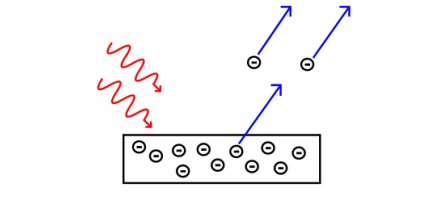
\includegraphics[width=.5\linewidth]{Images/EfectoFotoelectrico.png}
            \caption{}
      \end{center}
\end{figure}

% + -------------------------------------------------------------|>
\subsection{La constante de Planck~\cite{Belmonte_2022}}

La constante de Planck relaciona la energía de una
partícula a su longitud de onda y, por tanto, constituye la
magnitud fundamental de la mecánica cuántica que no se
utilizó solamente para hacer descubrimientos posteriores,
si no que es muy utilizada hoy en día en la práctica de
muchas ciencias. En la actualidad, esta constante es muy
utilizada en física para medir la energía de una radiación,
no solamente en una unidad de energía, sino también en
unidades de longitud y de frecuencia. La constante de
Planck es además, utilizada en el campo de la astronomía ya
que, al utilizar la ley del cuerpo negro, se puede
determinar la temperatura de un objeto cuya emisión está
centrada en cierta frecuencia.

\begin{equation*}
      E = hf
\end{equation*}

% ! ----------------------------------------------------------------------|>
\section{Montaje Experimental}

Materiales utilizados:

\begin{multicols}{2}
      \begin{itemize}[label=$\triangleright$]
            \item Celda fotoeléctrica
            \item Lámpara de mercurio de alta presión
            \item Electrómetro amplificador
            \item Voltímetro de CC
            \item Filtros de interferencia
      \end{itemize}
\end{multicols}

El experimento se llevó a cabo para verificar
experimentalmente la ecuación de Einstein para el efecto
fotoeléctrico. Se utilizó el siguiente montaje
experimental:

\begin{enumerate}
      \item Encender la lámpara de mercurio de alta presión, que emite
            luz de varias longitudes de onda.
      \item Dirigir la luz de la lámpara hacia la celda fotoeléctrica.
      \item Conectar la celda fotoeléctrica al electrómetro
            amplificador y al voltímetro de CC\@{}.
      \item Seleccionar diferentes filtros de interferencia para
            controlar la longitud de onda de la luz incidente.
      \item Registrar los valores de tensión límite ($V_0$)
\end{enumerate}

\begin{figure}[H]
      \begin{center}
            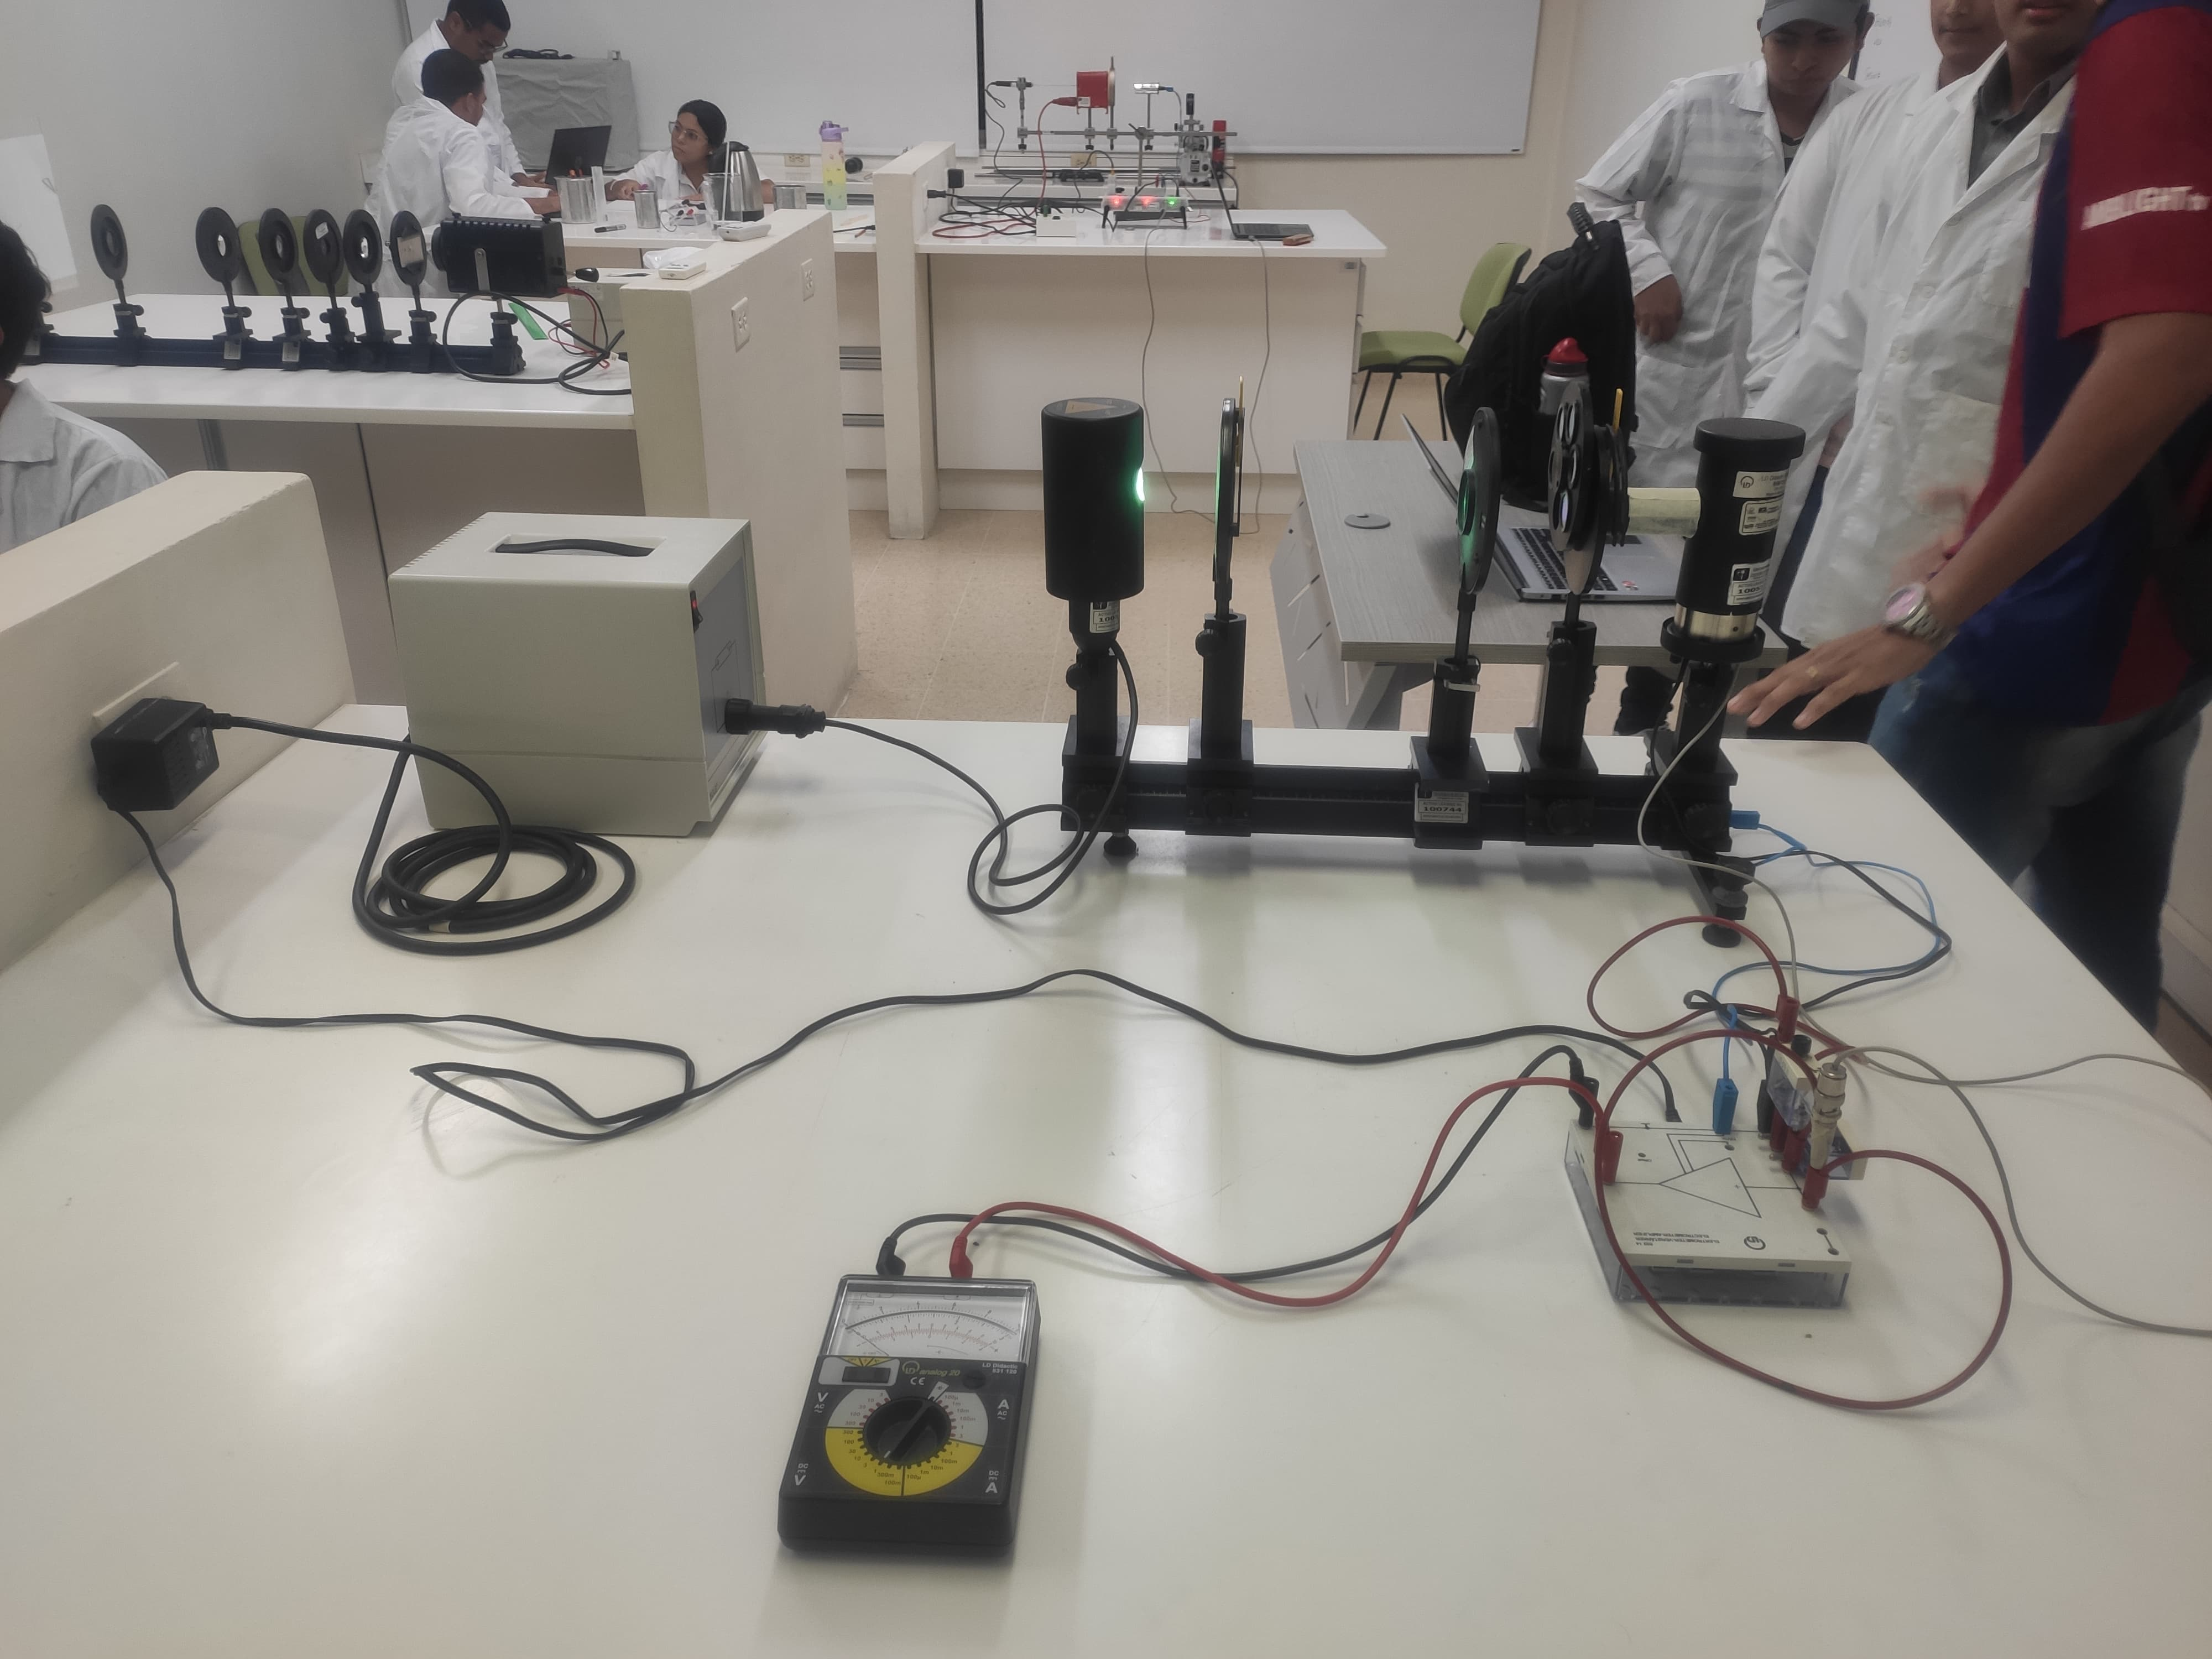
\includegraphics[width=.5\linewidth]{Images/MontajeExperimental.jpeg}
            \caption{}
      \end{center}
\end{figure}

% ! ----------------------------------------------------------------------|>
\section{Datos Experimentales}

\begin{table}[H]
      \begin{center}
            \begin{tabularx}{.9\linewidth}{|X|>{\centering\arraybackslash}X|>{\centering\arraybackslash}X|>{\centering\arraybackslash}X|}
                  \hline
                  \multicolumn{1}{|c|}{\multirow{2}{*}{\textbf{Lentes} \textit{(nm)}}} & \multicolumn{3}{c|}{\textbf{V}}                     \\
                  \cline{2-4}
                                                                                       & Grande                          & Mediano & Pequeño \\\hline
                  $365$                                                                & $1.700$                         & $1.600$ & $1.350$ \\\hline
                  $405$                                                                & $1.050$                         & $1.000$ & $0.850$ \\\hline
                  $436$                                                                & $0.800$                         & $0.720$ & $0.640$ \\\hline
                  $546$                                                                & $0.540$                         & $0.540$ & $0.500$ \\\hline
                  $578$                                                                & $0.440$                         & $0.340$ & $0.300$ \\\hline

            \end{tabularx}
      \end{center}
\end{table}

% ! ----------------------------------------------------------------------|>
\section{Análisis de datos}

% + -------------------------------------------------------------|>
\subsection{}

En este experimento, la tensión límite disminuyó cuando se
cambió la intensidad del haz incidente en la celda
fotoeléctrica. Esto indica que la intensidad del haz
(número de fotones) influye en la cantidad de energía
necesaria para liberar electrones y, por lo tanto, en la
tensión límite. Se logro notar que a medida que se
disminuyó la intensidad del haz incidente, disminuyó a su
vez la tensión, por lo que se puede afirmar que son
directamente proporcionales.

% + -------------------------------------------------------------|>
\subsection{}

Aplicando la formula,

\begin{equation*}
      f = \frac{c}{\lambda}
\end{equation*}

podemos obtener la frecuencia para cada $\lambda$, siendo
$c = 3 \times 10^{8}$ m/s

Basado en esto obtenemos,

\begin{table}[H]
      \begin{tabularx}{.9\linewidth}{|X|>{\centering\arraybackslash}X|X|>{\centering\arraybackslash}X|X|>{\centering\arraybackslash}X|X|>{\centering\arraybackslash}X|}
            \hline
            f                     & Pequeño & Mediano & Grande  \\\hline
            $8.22 \times 10^{14}$ & $1,350$ & $1,600$ & $1,700$ \\\hline
            $7.41 \times 10^{14}$ & $850$   & $1,000$ & $1,050$ \\\hline
            $6.88 \times 10^{14}$ & $640$   & $720$   & $800$   \\\hline
            $5.49 \times 10^{14}$ & $500$   & $540$   & $540$   \\\hline
            $5.19 \times 10^{14}$ & $300$   & $340$   & $440$   \\\hline
      \end{tabularx}
\end{table}

\begin{figure}[H]
      \begin{center}
            \includegraphics[width=.7\linewidth]{Images/AperturaPequeña.png}
            \caption{}
      \end{center}
\end{figure}

\begin{figure}[H]
      \begin{center}
            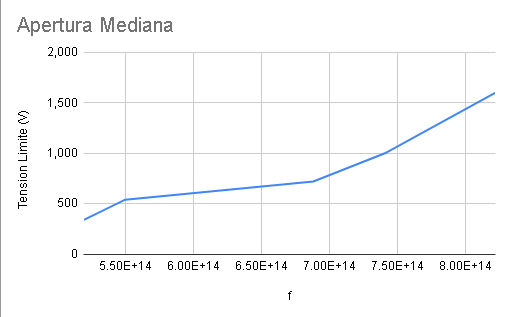
\includegraphics[width=.7\linewidth]{Images/AperturaMediana.png}
            \caption{}
      \end{center}
\end{figure}

\begin{figure}[H]
      \begin{center}
            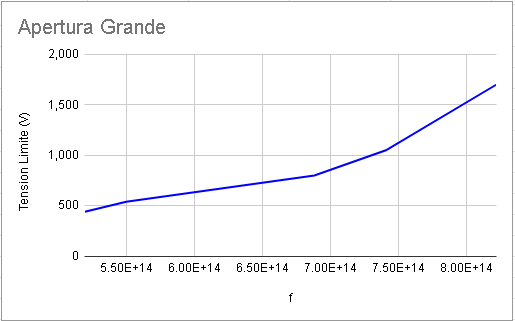
\includegraphics[width=.7\linewidth]{Images/AperturaGrande.png}
            \caption{}
      \end{center}
\end{figure}

% + -------------------------------------------------------------|>
\subsection{}

Aplicando regresión lineal encontramos

\begin{figure}[H]
      \begin{center}
            \includegraphics[width=.7\linewidth]{Images/TendenciaPequeña.png}
            \caption{$y = 2.95 \times 10^{-12}x - 1233$}
      \end{center}
\end{figure}

\begin{figure}[H]
      \begin{center}
            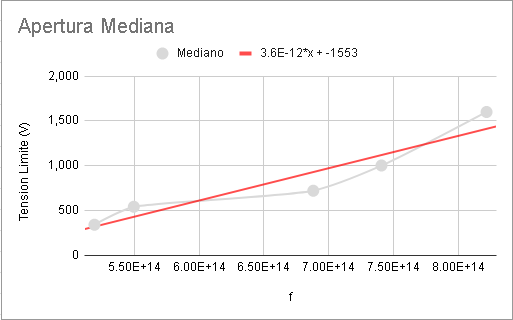
\includegraphics[width=.7\linewidth]{Images/TendenciaMediana.png}
            \caption{$y = 3.6 \times 10^{-12}x - 1553$}
      \end{center}
\end{figure}

\begin{figure}[H]
      \begin{center}
            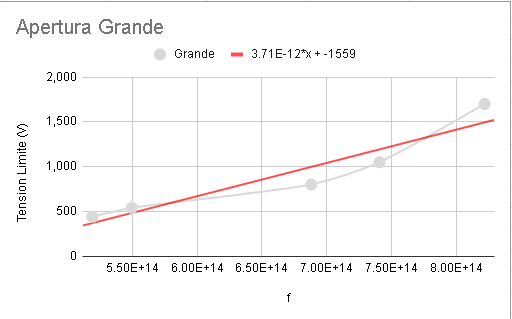
\includegraphics[width=.7\linewidth]{Images/TendenciaGrande.png}
            \caption{$y = 3.71 \times 10^{-12}x - 1559$}
      \end{center}
\end{figure}

% + -------------------------------------------------------------|>
\subsection{}

\begin{figure}[H]
      \begin{center}
            \includegraphics[width=.7\linewidth]{Images/SuperposicionPequeña.png}
            \caption{}
      \end{center}
\end{figure}

\begin{figure}[H]
      \begin{center}
            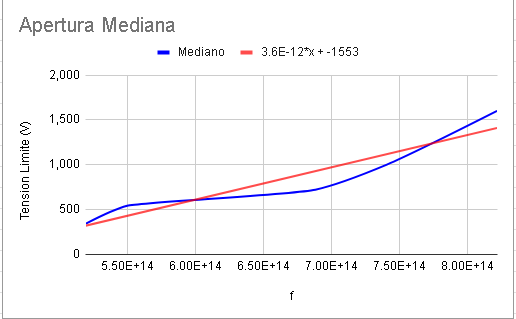
\includegraphics[width=.7\linewidth]{Images/SuperposicionMediana.png}
            \caption{}
      \end{center}
\end{figure}

\begin{figure}[H]
      \begin{center}
            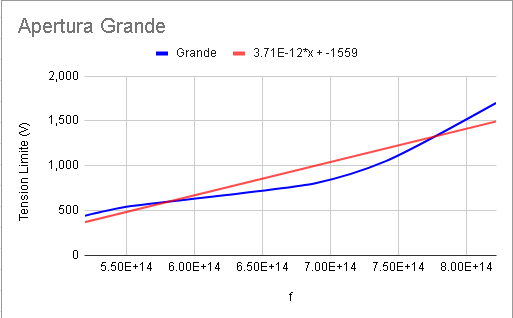
\includegraphics[width=.7\linewidth]{Images/SuperposicionGrande.png}
            \caption{}
      \end{center}
\end{figure}

% + -------------------------------------------------------------|>
\subsection{}

Primero se debe de encontrar la pendiente promedio entre
las ecuaciones:

\begin{equation*}
      \begin{gathered}
            y_{1} = 2.95 \times 10^{-12} x - 1233 \\
            y_{2} = 3.6 \times 10^{-12} x - 1533 \\
            y_3 = 3.71 \times 10^{-12} x - 1559
      \end{gathered}
\end{equation*}

\begin{equation*}
      m_{Promedio} = 3.42 \times 10^{-12}
\end{equation*}

\begin{enumerate}
      \item \begin{equation*}
                  y = mx + b \rightarrow V_{o} = \frac{h}{e}v - \frac{W_{o}}{e}
            \end{equation*}

            Donde la pendiente m esta relacionada a la ecuación
            $\frac{h}{e}$, donde $h$ es la constante de Planck

            \begin{equation*}
                  \begin{gathered}
                        m = \frac{h}{e} \rightarrow h = m \cdot e \\
                        h = (3.42 \times 10^{-12}) (1.6 \times 10^{-19}) \\
                        h = 5.472 \times 10^{-31} J/s
                  \end{gathered}
            \end{equation*}

      \item \begin{equation*}
                  \begin{gathered}
                        v = 6.638 \times 10^{14} Hz \\
                        W_{0} = 3,6323 \times 10^{-16} J
                  \end{gathered}
            \end{equation*}

      \item \begin{equation*}
                  \begin{gathered}
                        v = \frac{b}{m} \rightarrow v = \frac{h}{e \cdot m} \\
                        v = 0.9987 Hz
                  \end{gathered}
            \end{equation*}
\end{enumerate}

% ! ----------------------------------------------------------------------|>
\section{Conclusiones}

\printbibliography

\end{document}